\begin{frame}
\frametitle{Resumo do projeto}
\framesubtitle{Introdução}

\begin{figure}[hbt]
	\begin{center}
		\caption{Diagrama de bloco das etapas de desenvolvimento}
		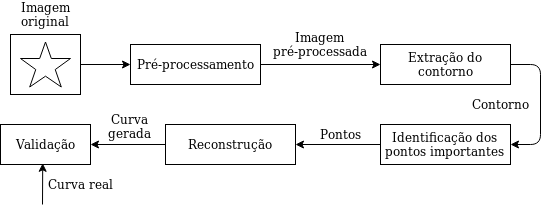
\includegraphics[width=1\textwidth]{img/diagrama.png}
	\end{center}
\end{figure}

\end{frame}


\begin{frame}
	\frametitle{Resumo do projeto}
	\framesubtitle{Exemplo (simples)}
	
	\begin{figure}[ht!]
		\centering
		\begin{subfigure}[b]{0.19\textwidth}
			\centering
			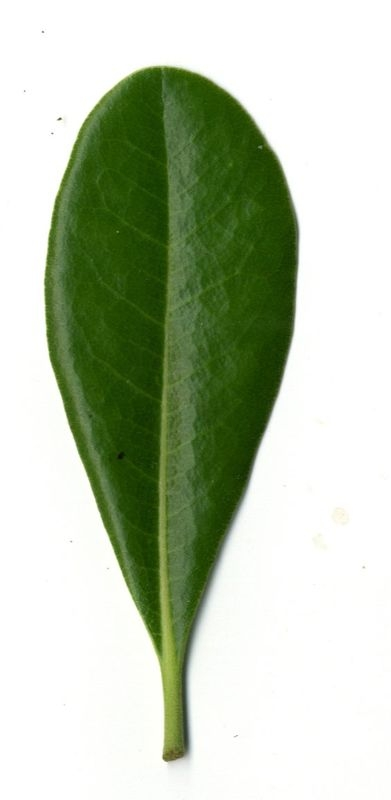
\includegraphics[width=\textwidth]{img/original.jpg}
		\end{subfigure}
		\begin{subfigure}[b]{0.19\textwidth}
			\centering
			
\includegraphics[width=\textwidth]{img/preprocess.jpg}
		\end{subfigure}
		\begin{subfigure}[b]{0.19\textwidth}
			\centering
			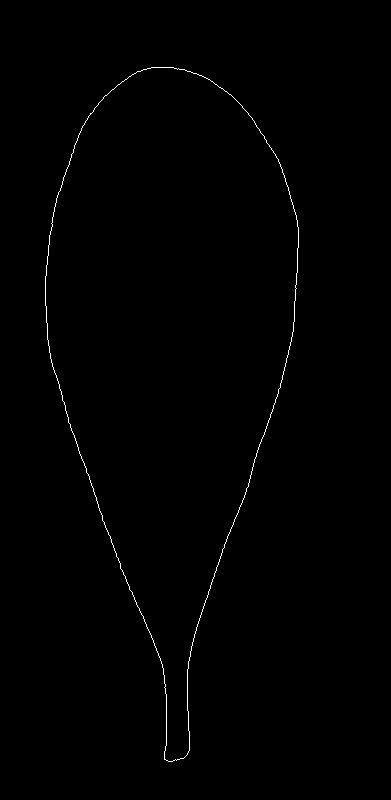
\includegraphics[width=\textwidth]{img/contour.jpg}
		\end{subfigure}
		\begin{subfigure}[b]{0.19\textwidth}
			\centering
			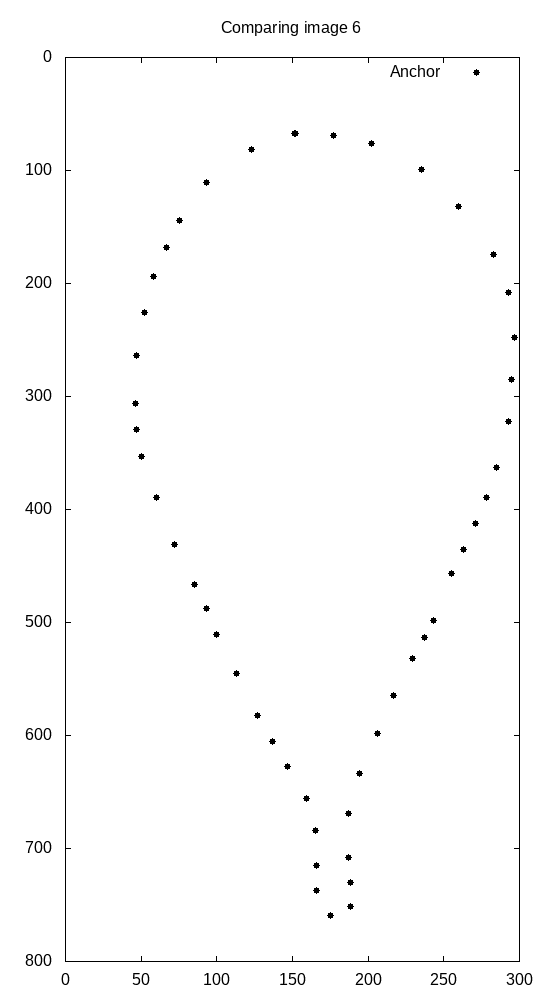
\includegraphics[width=\textwidth]{img/points.png}
		\end{subfigure}
		\begin{subfigure}[b]{0.19\textwidth}
			\centering
			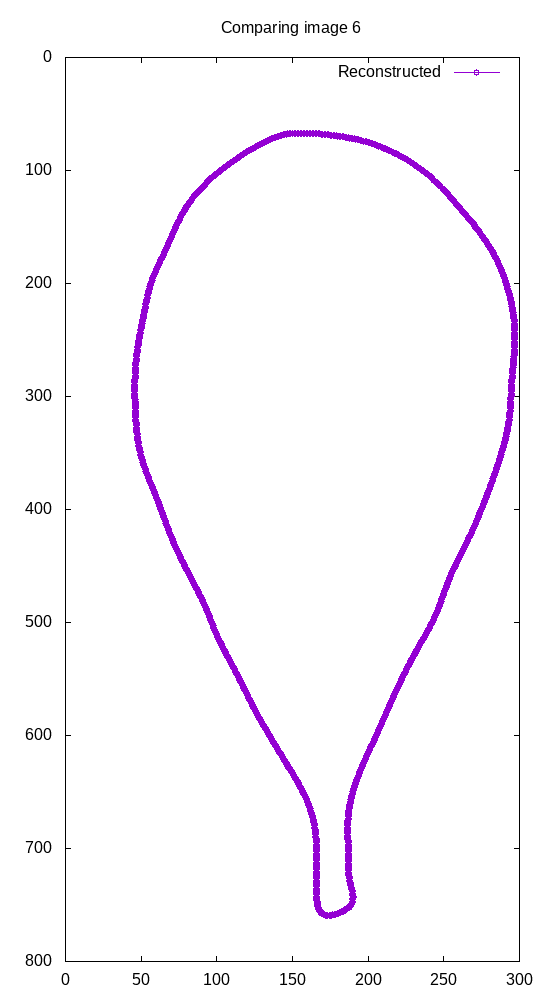
\includegraphics[width=\textwidth]{img/reconstructed.png}
		\end{subfigure}
		\label{fig:editedmesh}
	\end{figure}
	
\end{frame}


